%\begin{figure}
%	\section{Robot 9} %cambiar titulo
%	\centering	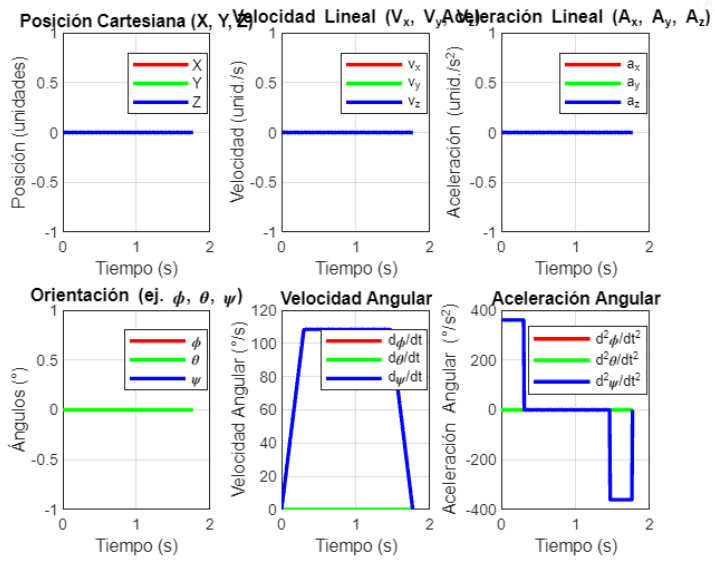
\includegraphics[width=0.8\linewidth]{img/robot9_1}
%	\caption{} %cambiar pie de imagen
%	\label{fig:robot9}
%\end{figure}
%
%
%\begin{figure}
%	\centering	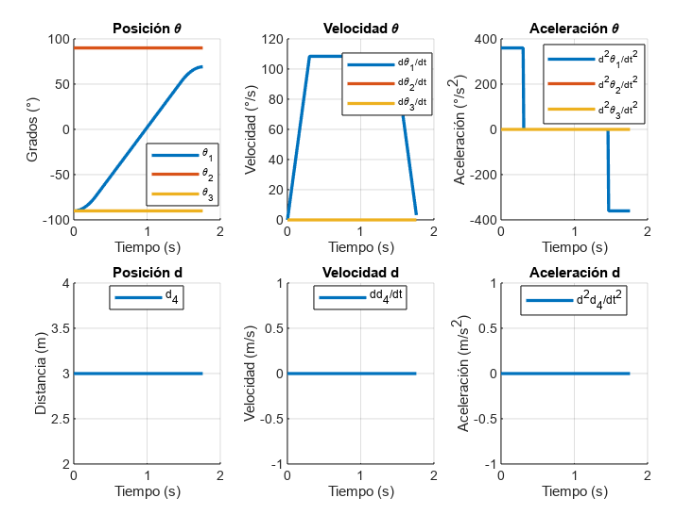
\includegraphics[width=0.8\linewidth]{img/robot9_2}
%	\caption{} %cambiar pie de imagen
%	\label{fig:robot_9}
%\end{figure}
%
%
%\begin{figure}
%	\centering	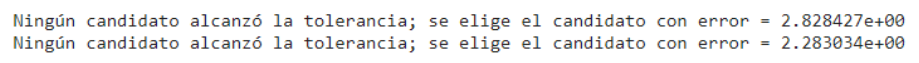
\includegraphics[width=0.8\linewidth]{img/robot9_3}
%	\caption{Error del objetivo} %cambiar pie de imagen
%	\label{fig:robot_9_error}
%\end{figure}
\begin{figure}[h]
	\section{Robot 9} 
	\centering
	\subfloat[]{%
		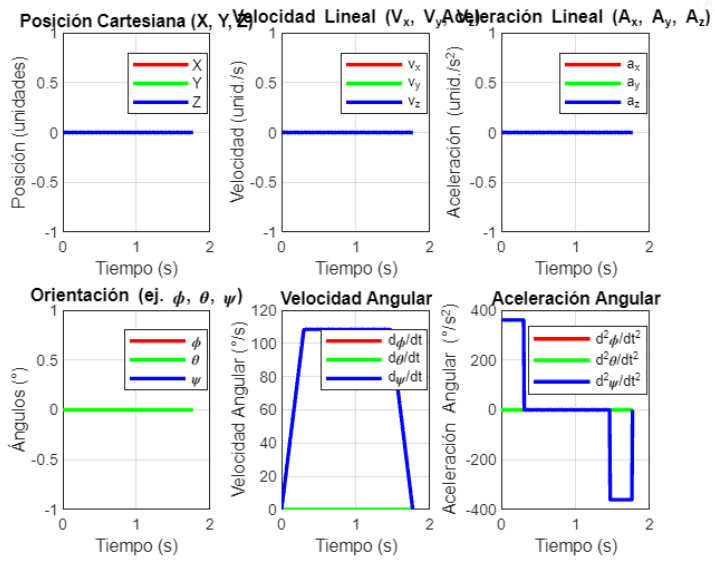
\includegraphics[width=0.75\textwidth]{img/robot9_1}%
		\label{fig:robo9_1}
	}
	\hfill
	\subfloat[]{%
		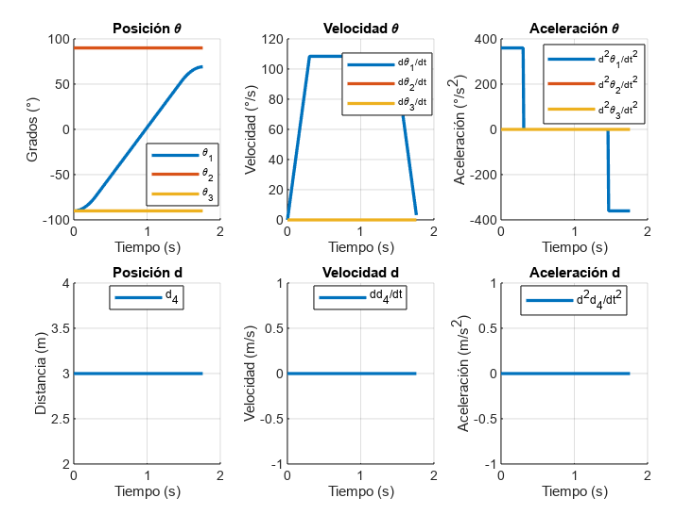
\includegraphics[width=0.75\textwidth]{img/robot9_2}%
		\label{fig:robot9_2}
	}
	\hfill
	\subfloat[Error del objetivo]{%
		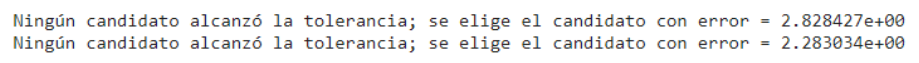
\includegraphics[width=0.8\textwidth]{img/robot9_3}%
		\label{fig:robot9_3}
	}
	\caption{Robot 9}
	\label{fig:Robot9}
\end{figure}